% Fase 3B, exemplos 9–10. Fontes: mb-uso/secoes.
\begin{frame}[fragile]{Exemplo 9 — Reanalisar dados sem repetir a otimização}
\begin{columns}[T,onlytextwidth]
\begin{column}{.49\textwidth}
\begin{lstlisting}[style=python,basicstyle=\ttfamily\fontsize{7.5}{9.5}\selectfont]
exp.run(repeat=3)
exp.save('study_full', mode='all')
exp.save('study_config',mode='config')

restored = mb.experiment()
restored.load('study_full', mode='all')

loaded = mb.experiment()
loaded.mop = mb.mops.DTLZ2(M=2)
loaded.load('study_full', mode='data')
mb.view.topology(loaded)
\end{lstlisting}
\end{column}
\begin{column}{.49\textwidth}
\textbf{O que é preservado?}
\par\smallskip
\texttt{all}: configuração \textbf{e} dados.
\par\smallskip
\texttt{config}: apenas o protocolo para reprodução.
\par\smallskip
\texttt{data}: recuperação dos resultados em um objeto já configurado.
\par\medskip
Não é preciso consumir novamente o orçamento de avaliações para gerar uma nova análise dos dados armazenados.
\end{column}
\end{columns}
\end{frame}

\begin{frame}[fragile]{Exemplo 9 — A figura usa resultados recuperados do arquivo}
\begin{columns}[T,onlytextwidth]
\begin{column}{.64\textwidth}
\centering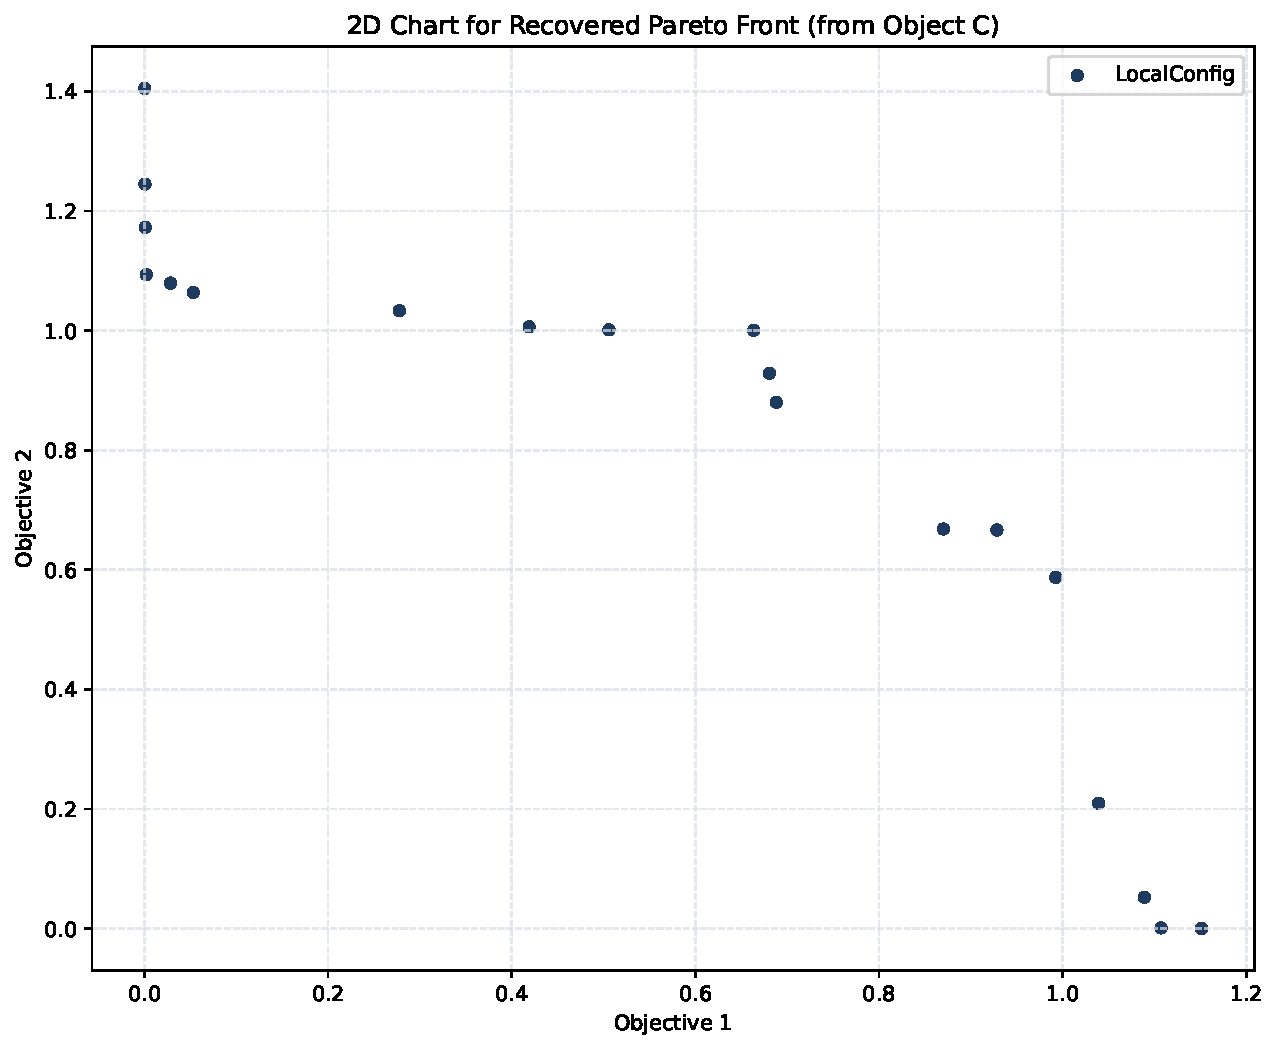
\includegraphics[width=\linewidth,height=.62\textheight,keepaspectratio]{figures/example_09_01_topology.pdf}
\end{column}
\begin{column}{.34\textwidth}
\textbf{DTLZ2 bidimensional, 3 execuções.}
\par\smallskip
Populações finais reunidas: \textbf{60 soluções}.
\par\smallskip
Não dominadas no conjunto: \textbf{22}.
\par\medskip
A figura foi produzida após o carregamento, e não a partir de uma nova execução do algoritmo.
\end{column}
\end{columns}
\vspace{.04cm}\textbf{Interpretação:} reprodutibilidade do protocolo e preservação dos resultados são operações distintas; o experimento pode ser reanalisado sem recomputar a otimização.
\end{frame}

\begin{frame}[fragile]{Exemplo 10 — Objetivos similares implicam decisões similares?}
\textbf{Protocolo:} NSGA-II versus NSGA-III no DTLZ2 com 3 objetivos e 12 variáveis de decisão.
\begin{columns}[T,onlytextwidth]
\begin{column}{.56\textwidth}
\begin{lstlisting}[style=python,basicstyle=\ttfamily\fontsize{7.3}{9.1}\selectfont]
a = mb.stats.topo_match(
    exp1, exp2, alpha=0.01)
b = mb.stats.topo_match(
    exp1, exp2, space='vars')
c = mb.stats.topo_shift(
    exp1, exp2, method='emd',
    threshold=0.05)
a.report(); b.report(); c.report()
mb.view.density(exp1,exp2,space='objs')
mb.view.density(exp1,exp2,space='vars')
\end{lstlisting}
\end{column}
\begin{column}{.42\textwidth}
\textbf{Testes KS dos objetivos:}
\par $p=(0{,}4440,\;0{,}5603,\;0{,}1648)$.
\par\smallskip
Nenhum está abaixo de $\alpha=0{,}01$.
\par\medskip
\textbf{Decisões:} seis das 12 variáveis diferem entre algoritmos ($\alpha=0{,}05$ no relatório).
\end{column}
\end{columns}
\vspace{.06cm}\textbf{Conclusão:} resultados aparentemente semelhantes nos objetivos não exigem que os MOEAs utilizem as mesmas regiões do espaço de decisões.
\end{frame}

\begin{frame}{Exemplo 10 — As densidades mostram o contraste entre espaços}
\centering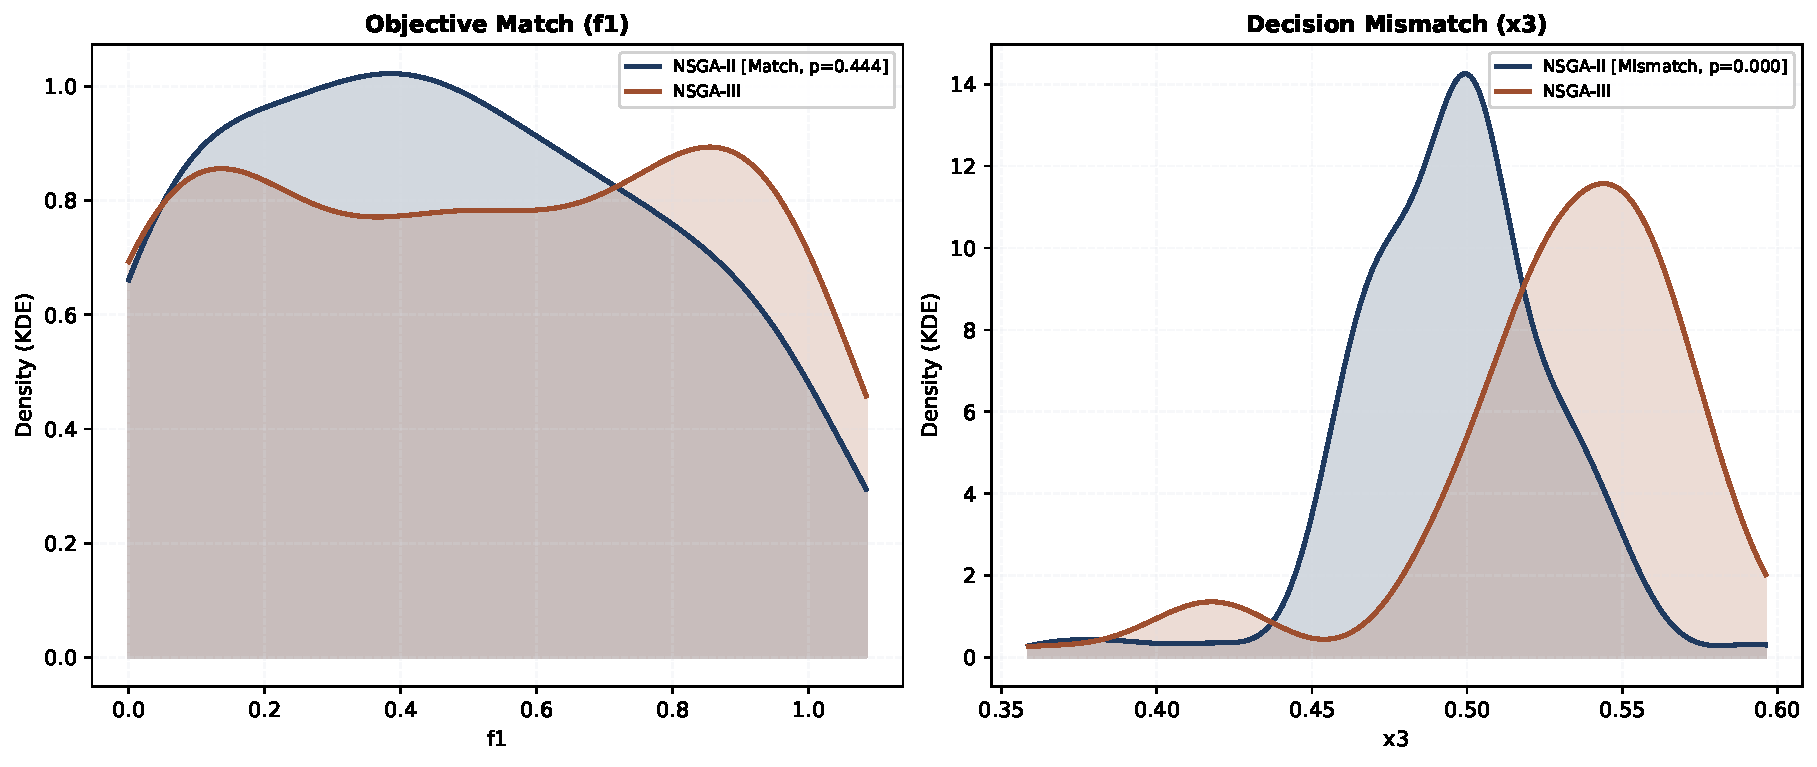
\includegraphics[width=.97\linewidth,height=.45\textheight,keepaspectratio]{figures/example_10_composite_01.pdf}
\par\smallskip
\textbf{Esquerda, objetivo $f_1$:} as distribuições apresentam ampla sobreposição. \textbf{Direita, variável $x_3$:} as densidades se separam visivelmente.
\par\smallskip
\textbf{EMD nos objetivos:} $0{,}0553$, $0{,}0523$ e $0{,}0524$, pouco acima de $0{,}05$. O EMD identifica diferenças que não se destacaram nos testes KS nesse critério.
\end{frame}
